\begin{figure}[htbp]
\centering
\begin{adjustbox}{max width=\textwidth,center}
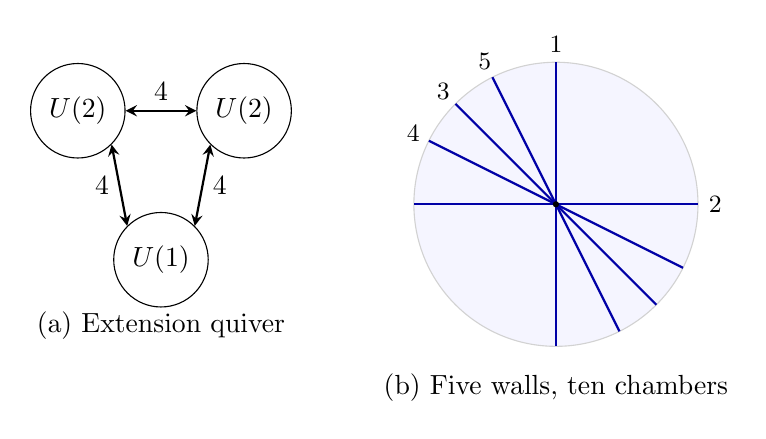
\begin{tikzpicture}[scale=.88,>=stealth]
 \node[circle,draw,minimum size=12mm] (v1) at (-4.7,1.6) {$U(2)$};
 \node[circle,draw,minimum size=12mm] (v2) at (-2.3,1.6) {$U(2)$};
 \node[circle,draw,minimum size=12mm] (v3) at (-3.5,-.55) {$U(1)$};
 \draw[<->,thick] (v1.east)--node[above]{$4$}(v2.west);
 \draw[<->,thick] (v1.south east)--node[left]{$4$}(v3.north west);
 \draw[<->,thick] (v2.south west)--node[right]{$4$}(v3.north east);
 \node at (-3.5,-1.5) {(a) Extension quiver};
 \begin{scope}[xshift=2.2cm,yshift=.25cm]
  \fill[blue!4] (0,0) circle[radius=2.05];
  \draw[gray!35] (0,0) circle[radius=2.05];
  \foreach \ang in {0,90,116.565051,135,153.434949}
    \draw[blue!65!black,thick] (\ang:2.05)--(\ang+180:2.05);
  \fill (0,0) circle[radius=.045];
  \node[font=\small] at (90:2.3) {$1$};
  \node[font=\small] at (0:2.3) {$2$};
  \node[font=\small] at (135:2.3) {$3$};
  \node[font=\small] at (153.434949:2.3) {$4$};
  \node[font=\small] at (116.565051:2.3) {$5$};
  \node at (0,-2.65) {(b) Five walls, ten chambers};
 \end{scope}
\end{tikzpicture}
\end{adjustbox}
\caption{The rank-five example. Each edge in (a) denotes four arrows in
each direction; the diagonal circle acts trivially. In (b) the horizontal
and vertical coordinates are $\zeta_1,\zeta_2$. Wall numbers refer to
Table~\ref{tab:walls}; the bounding circle has no geometric significance.}
\label{fig:quiver-walls}
\end{figure}

